\subsection{Equazioni Neurali Differenziali}

Sin dalla pubblicazione dell'articolo di Chen et al. (2019) 
\cite{chen2019neural}, la tecnica delle Equazioni Neurali Differenziali 
(END) ha attirato notevole attenzione, portando all'ibridazione di due 
paradigmi di modellazione distinti: le Equazioni Differenziali Ordinarie 
(ODE) e le reti neurali (NN). Questo sforzo mira a sfruttare al meglio 
entrambi i paradigmi, minimizzando gli effetti indesiderati \cite{chen2019neural} \cite{Kim_2021}.

Un'Equazione Differenziale è un metodo per specificare una trasformazione 
non lineare arbitraria, codificando matematicamente le ipotesi strutturali 
a priori del sistema. Esistono tre approcci comuni per definire tale 
trasformazione non lineare:

\begin{itemize}
    \item \textbf{Modellazione diretta}
    \item \textbf{Machine learning}
    \item \textbf{Equazioni differenziali}
\end{itemize}

L'approccio di modellazione diretta funziona solo quando si conosce 
la funzione esatta che collega l'input con l'output. Tuttavia, nella 
maggior parte dei casi, questa relazione è sconosciuta a priori, 
rendendo impossibile applicare questo metodo. In questi casi, l'approccio 
di machine learning diventa una soluzione valida.

\begin{minipage}{\linewidth}
    \centering
    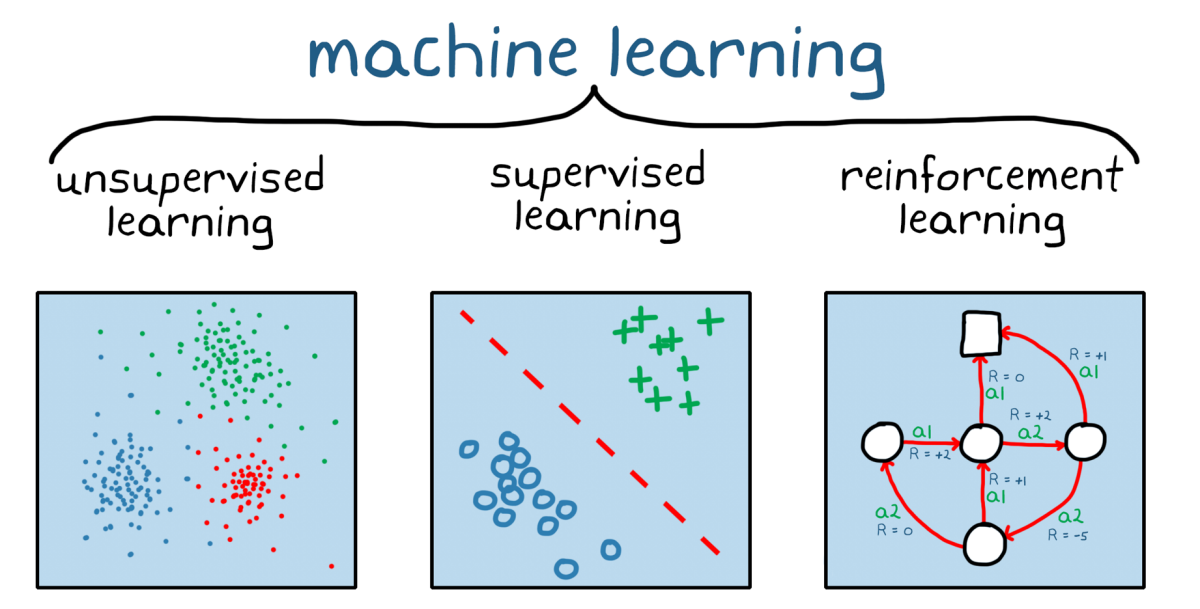
\includegraphics[width=\textwidth]{img/1689243301131.png}
    \captionof{figure}{Differenti approcci di apprendimento di machine learning}
    \url{https://it.mathworks.com/discovery/reinforcement-learning/_jcr_content/mainParsys3/discoverysubsection/mainParsys/image.adapt.full.medium.png/1689243301131.png}
    \label{fig:ML_example}
\end{minipage}

Nel contesto generale del machine learning, dato un insieme di dati $x$, 
l'obiettivo è predire un insieme $y$ di dati correlati utilizzando una 
funzione sottostante. Questa funzione viene comunemente chiamata "modello". 
Si inizia con una fase di addestramento in cui si cercano di regolare i 
parametri (iperparametri) del modello per ottenere un modello in grado di 
generare previsioni accurate. Successivamente, il modello viene utilizzato 
per inferire dati $x$ mai visti in precedenza. In sostanza, questo 
approccio consiste in una serie di trasformazioni non lineari.

L'uso del machine learning è affascinante perché si basa su un concetto 
estremamente semplice ma potente: adattare il modello ai dati forniti in 
modo efficace. Questa idea si estende ulteriormente alle reti neurali (NN), 
che sono essenzialmente insiemi di moltiplicazioni tra matrici seguite 
dall'applicazione di una funzione di attivazione. Ad esempio, una 
semplice rete neurale a tre strati è definita come:

$$ML(x) = \sigma(W_3 \cdot \sigma(W_2 \cdot \sigma(W_1 \cdot x)))$$

Dove $W_1$, $W_2$, e $W_3$ sono parametri apprendibili. L'obiettivo è 
selezionare questi parametri in modo che $ML(x) = y$ si comporti in modo 
simile alla funzione incognita che si desidera adattare. Grazie 
all'applicazione del teorema di approssimazione universale, si afferma 
che con un numero sufficientemente grande di parametri o strati, è 
possibile approssimare qualsiasi funzione non lineare in modo 
sufficientemente preciso.

\begin{minipage}{\linewidth}
    \centering
    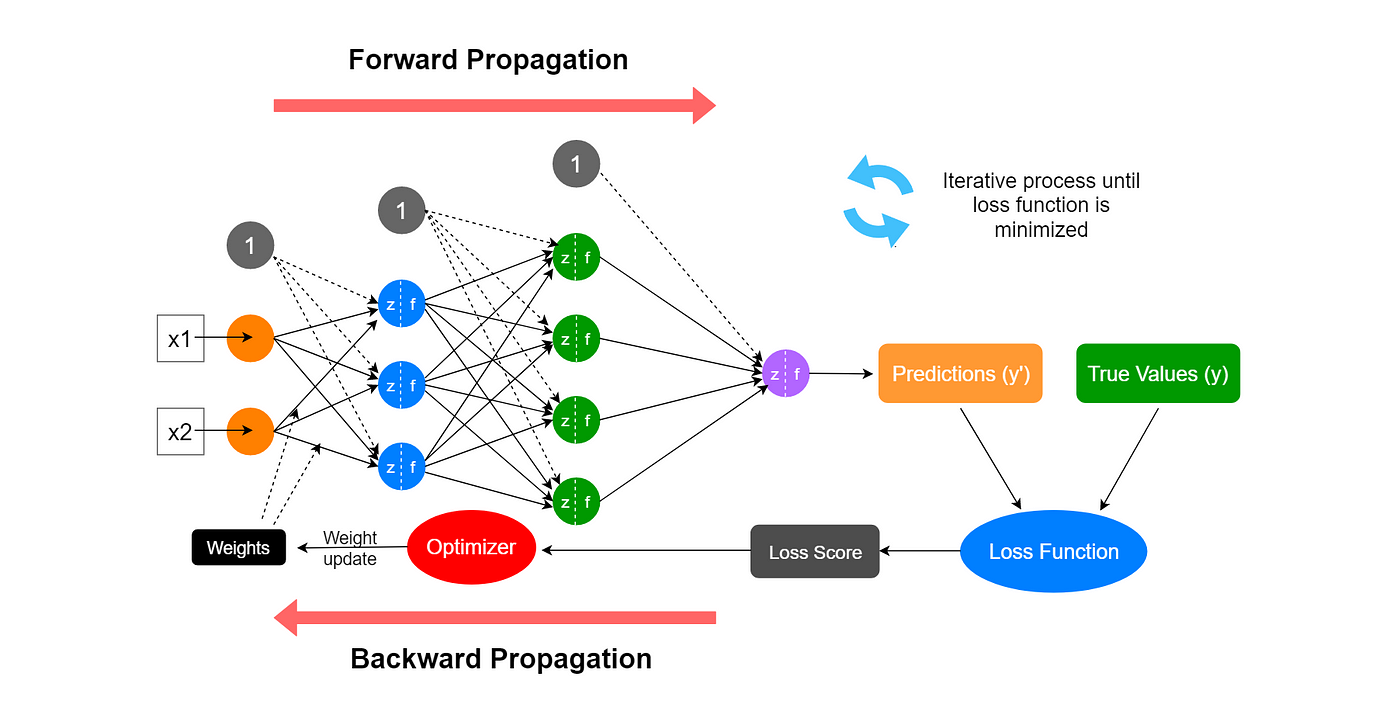
\includegraphics[width=\textwidth]{img/1_ZXAOUqmlyECgfVa81Sr6Ew.png}
    \captionof{figure}{Esempio di funzionamento di una rete neurale}
    \url{https://miro.medium.com/v2/resize:fit:4800/format:webp/1*ZXAOUqmlyECgfVa81Sr6Ew.png}
    \label{fig:NN_example}
\end{minipage}

Questo approccio richiede l'apprendimento di ogni aspetto della 
trasformazione non lineare direttamente dai dati disponibili. 
In molti casi, però, non è possibile conoscere l'intera equazione non 
lineare, ma forse se ne conosce la struttura generale. Un modo per 
definire matematicamente questo tipo di approccio è attraverso le 
equazioni differenziali. Un metodo immediato è quello di definire un 
modello matematico in cui si cerca di apprendere una costante associata al 
comportamento di un insieme di dati:

$$y'(t) = \alpha \cdot y(t)$$

Questo approccio non richiede la conoscenza della soluzione dell'equazione 
differenziale per convalidare la correttezza del modello. La struttura del 
modello e la matematica stessa sono incorporate nel modello stesso, il 
quale successivamente produce una soluzione. Questo tipo di modelli è 
essenzialmente un insieme di equazioni che descrivono il cambiamento 
delle variabili nel tempo, con la soluzione dell'equazione differenziale 
come risultato finale.

\begin{minipage}{\linewidth}
    \centering
    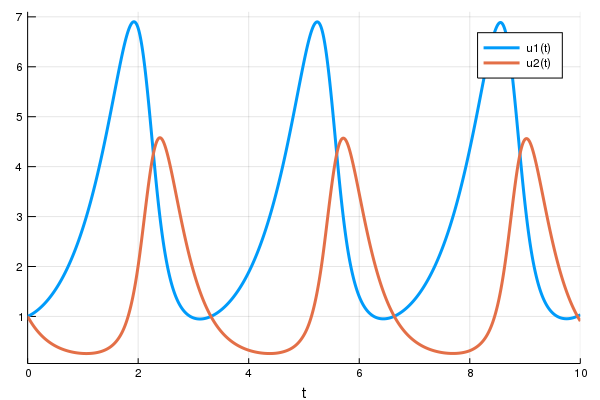
\includegraphics[width=\textwidth]{img/lotkavolterra.png}
    \captionof{figure}{Esempio grafico ODE rappresentante la famosa equazione di Lotka-Volterra}
    \label{fig:lotkavolterra_example}
\end{minipage}

Questo metodo è stato ampiamente utilizzato in campi scientifici, e 
recentemente ha visto ulteriori sviluppi tramite l'integrazione di 
strutture matematiche aggiuntive che permettono di modellare sistemi 
complessi come quelli in ambito farmacologico o biologico.

Ciò che rende i modelli di machine learning interessanti è la loro fame 
di dati e la necessità di un grande insieme di dati di allenamento. 
In questo contesto, l'uso delle equazioni differenziali è diventato 
una scelta interessante per specificare la non linearità in modo 
apprendibile (tramite parametri) in modo più efficiente. Questo permette 
di incorporare la conoscenza specifica di un dominio nelle relazioni 
strutturali tra input e output del modello.

Un'Equazione Differenziale Neurale (Neural ODE) rappresenta un modo per 
collegare i mondi del machine learning e delle equazioni differenziali. 
L'approccio generale è quello di non apprendere solo la trasformazione 
non lineare tra i dati, ma anche la struttura stessa della 
trasformazione non lineare. Invece di avere il modello $y = ML(x)$, 
si ha il modello $y' = ML(x)$, e successivamente si tenta di risolvere 
l'equazione differenziale associata.

L'approccio fondamentale qui è che definendo il modello in questo modo e 
utilizzando un risolutore semplice e propenso agli errori come il metodo 
di Euler, è possibile ottenere risultati equivalenti a quelli ottenuti 
con una ResNet \cite{he2015deep}. L'idea di base è che invece di 
modellare una rete neurale con sempre più strati, diventando sempre 
più profonda, è sufficiente modellare direttamente il sistema di 
equazioni differenziali e risolverlo con un risolutore specifico.

Questo approccio è efficiente dal punto di vista della memoria, è in 
grado di gestire dati irregolari, ha una forte conoscenza a priori 
dello spazio del modello, è in grado di approssimare sia funzioni 
lineari che non lineari e si basa su solide basi teoriche derivanti da 
entrambi i lati.

\subsubsection*{Risolvere un'ODE in Julia}

L'idea di base è quella di definire un oggetto "ODEProblem" specificando 
una funzione che descrive il sistema di ODE attraverso la specifica 
delle derivate delle equazioni nella forma $u' = f(u, p, t)$, fornendo 
un set di condizioni iniziali $u0$, un intervallo di tempo $t$, e un 
insieme di parametri $p$.

\begin{minipage}{\linewidth}
    \centering
    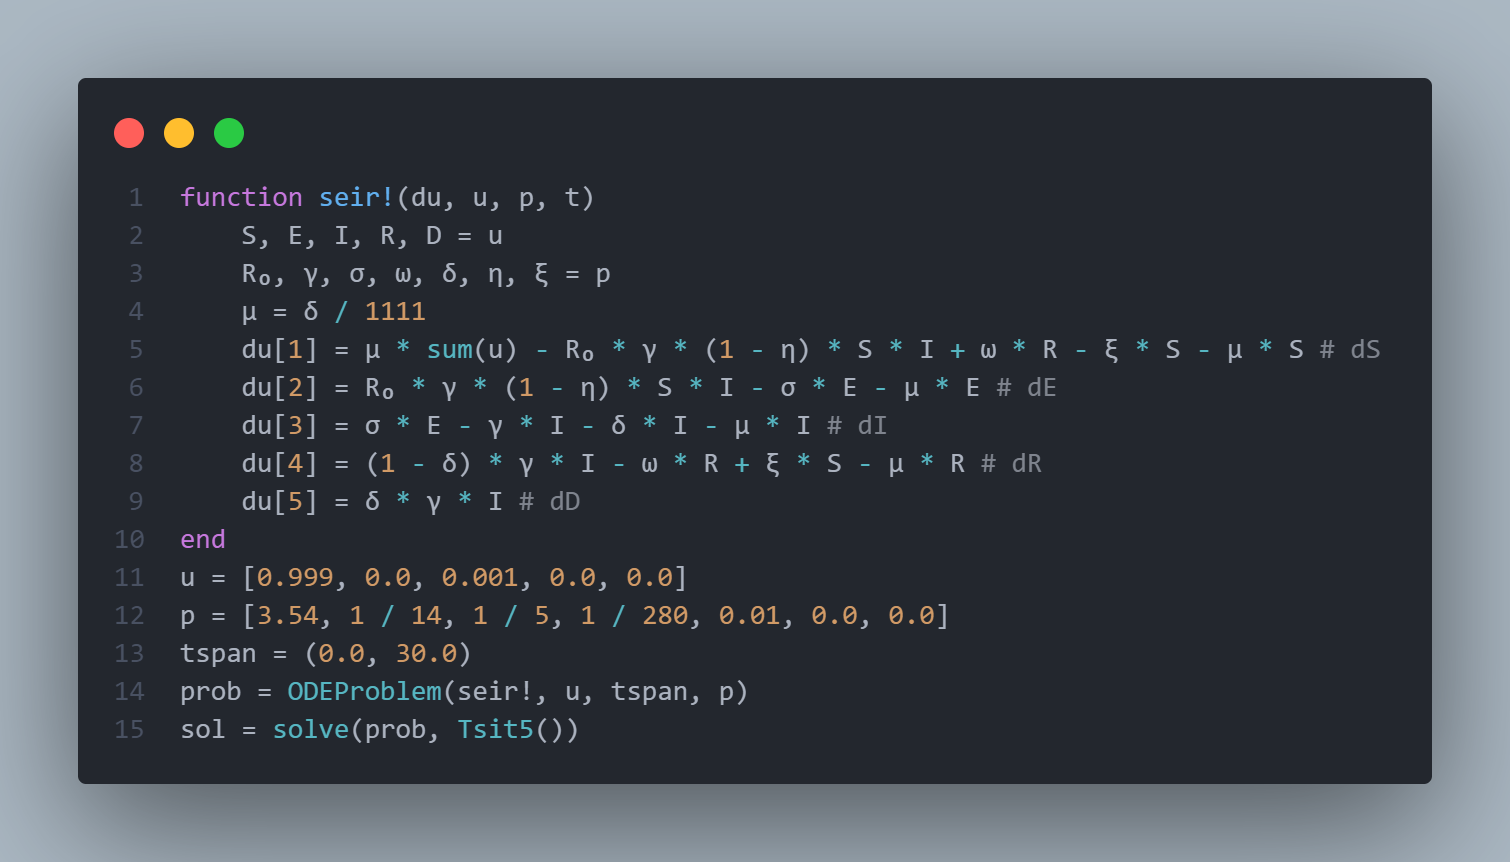
\includegraphics[width=\textwidth]{img/fdefinition.png}
    \captionof{figure}{Esempio definizione ODE in Julia}
    \label{fig:ODE_Julia_example}
\end{minipage}

Successivamente, è possibile risolvere il sistema di ODE utilizzando la 
funzione "solve". È possibile specificare diversi metodi per la 
risoluzione del sistema. Ad esempio, il metodo "Tsit5" è un metodo 
esplicito di quinto ordine di tipo Runge-Kutta con un stimatore di 
errore integrato di tipo Tsitouras \cite{10.1016/j.camwa.2011.06.002}. 
La libreria DifferentialEquations.jl offre una vasta gamma di parametri 
aggiuntivi per un approccio più dettagliato \cite{rackauckas2017differentialequations}.

\subsubsection{Inserire un'ODE all'interno di una NN}

Per capire meglio cosa significhi inserire un'ODE all'interno di una 
rete neurale (NN), è necessario esaminare come è definito un layer di 
una NN. Un layer è essenzialmente una funzione differenziabile che 
accetta un vettore di dimensione $n$ come input e restituisce un nuovo 
vettore di dimensione $m$ come output. Questo si allinea con l'idea che 
i risolutori di DE rientrano nella categoria delle funzioni 
differenziabili, il che significa che possono essere incorporati 
direttamente in un programma più grande basato su differenziazione 
automatica, come una rete neurale \cite{Flux.jl-2018} \cite{pal2023lux}. 

\begin{minipage}{\linewidth}
    \centering
    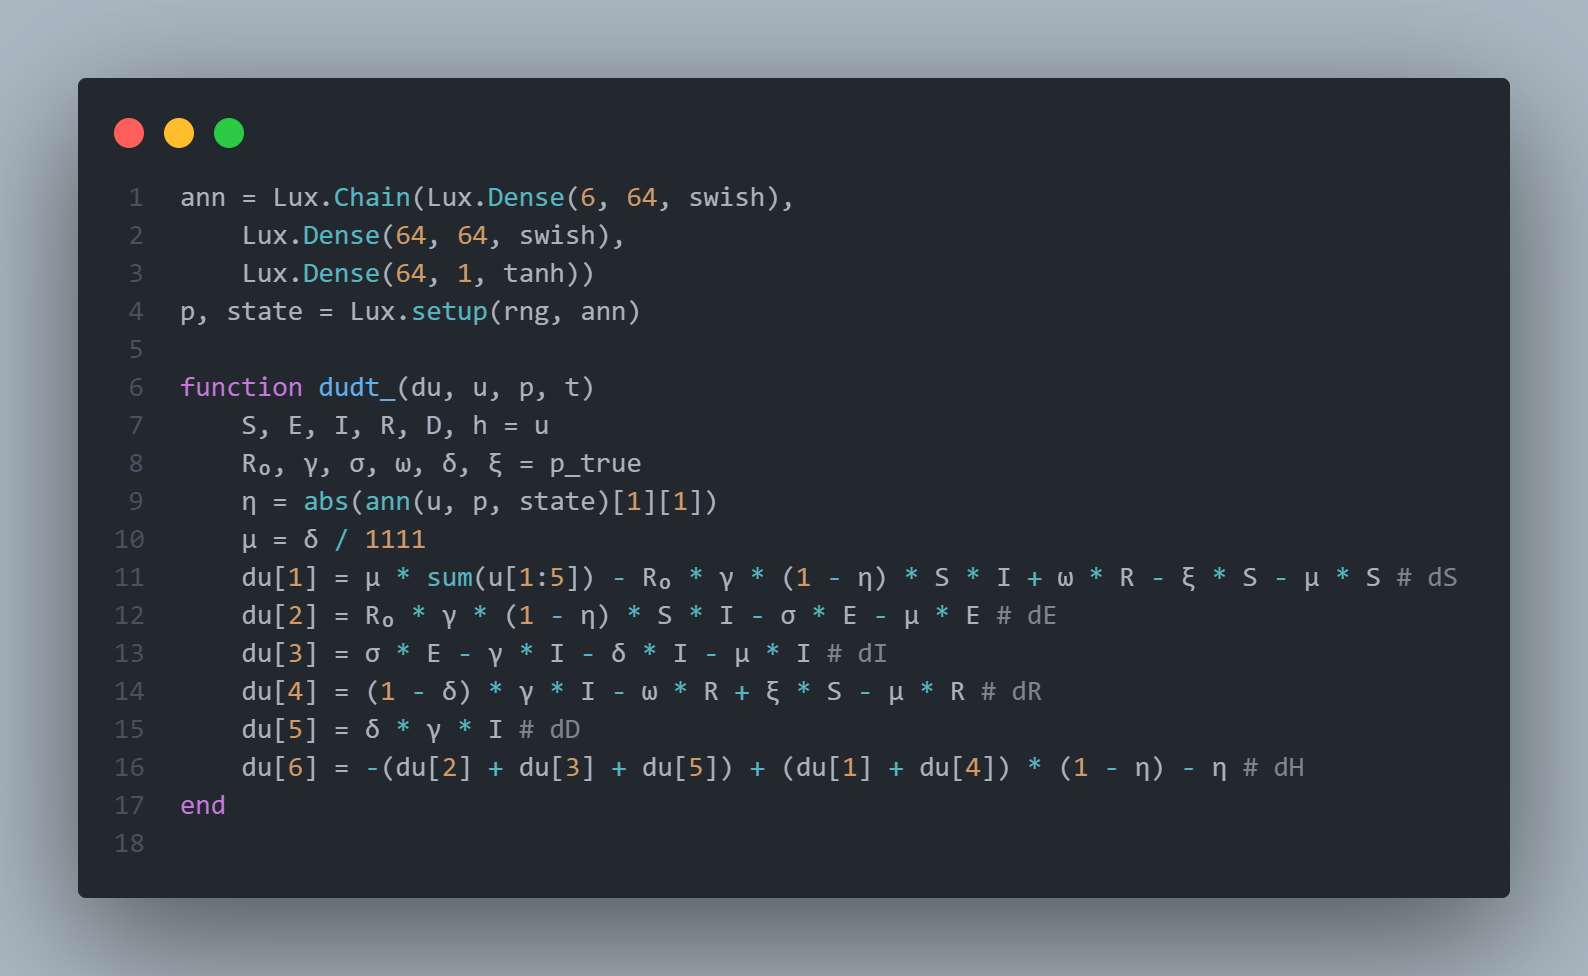
\includegraphics[width=\textwidth]{img/fann.png}
    \captionof{figure}{Esempio implementazione di una rete neurale in Julia}
    \label{fig:NN_Julia_example}
\end{minipage}

Successivamente, è possibile addestrare la NN per un numero specifico di 
integrazioni per ottenere i risultati desiderati. È importante 
sottolineare che il sistema non sta apprendendo una soluzione 
all'equazione differenziale, ma piuttosto sta apprendendo il sistema di 
equazioni differenziali da cui è generata la soluzione. La NN sta 
effettivamente apprendendo una rappresentazione compatta del comportamento 
della serie di dati nel tempo e può estrapolare facilmente cosa 
potrebbe accadere con diverse condizioni iniziali. La suite DiffEqFlux.jl 
offre un wrapper comodo per definire una "NeuralODE" \cite{rackauckas2019diffeqflux}.

\begin{minipage}{\linewidth}
    \centering
    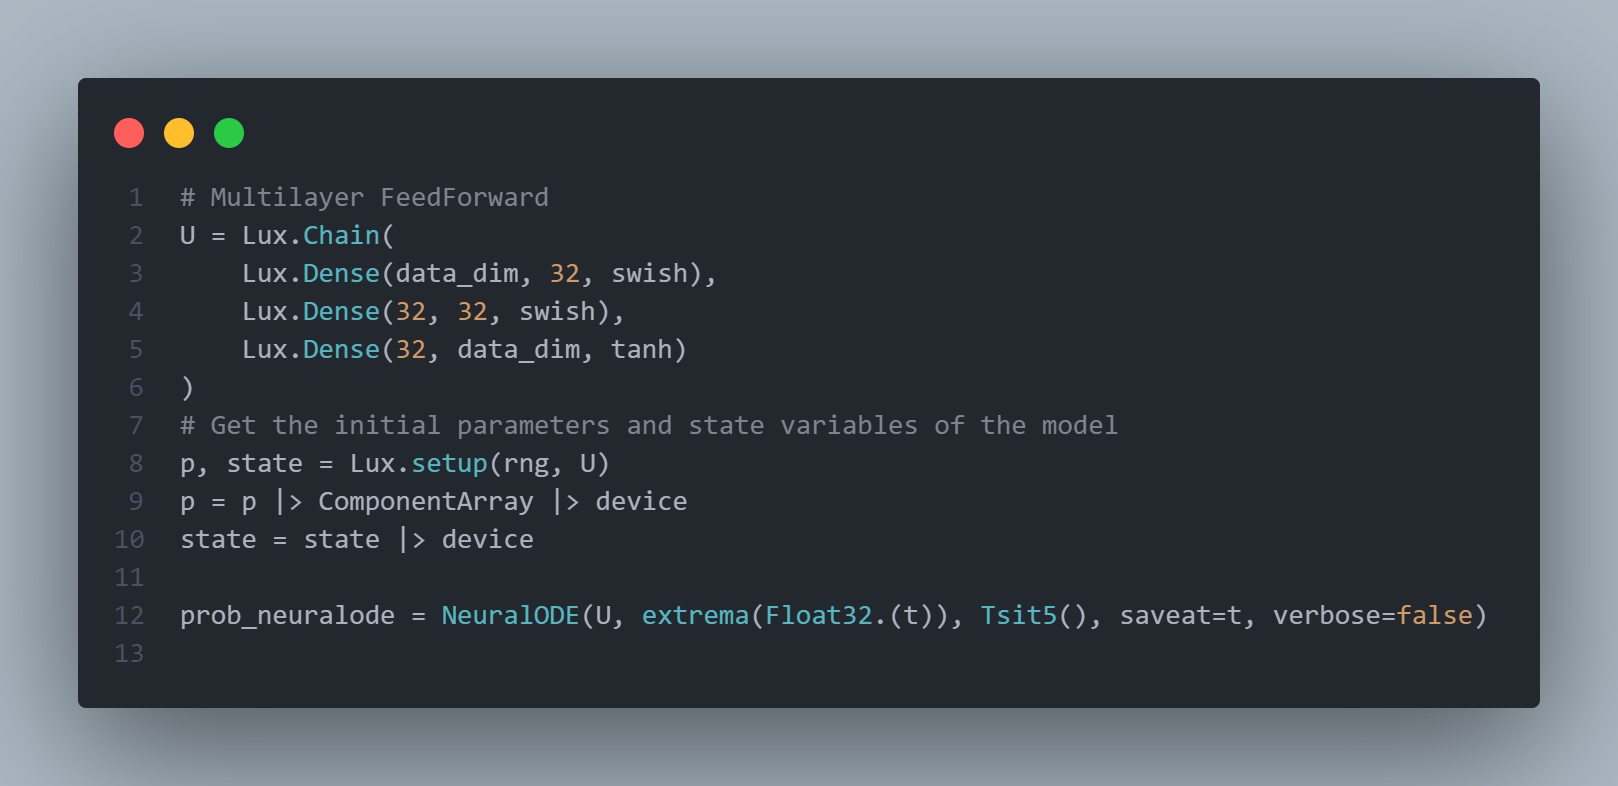
\includegraphics[width=0.8\textwidth]{img/fneuralode.png}
    \captionof{figure}{Esempio implementazione NeuralODE tramite DiffEqFlux.jl}
    \label{fig:NeuralODE_Julia_example}
\end{minipage}

\subsubsection{Backpropagation tramite ODE solver}

Il cuore di ogni rete neurale è la capacità di propagare all'indietro 
le derivate lungo l'intera rete per calcolare il gradiente della 
funzione di perdita rispetto ai parametri della rete. La sfida sta nel 
trovare un modo per applicare lo stesso principio quando si utilizzano 
risolutori di ODE all'interno di una rete neurale.

Esistono vari approcci per affrontare questo problema, ma il più comune 
è attraverso l'analisi di sensitività (adjointed). Questo approccio 
definisce una nuova ODE il cui obiettivo è calcolare il gradiente della 
funzione di costo rispetto ai parametri e successivamente risolvere 
questa seconda ODE.

L'approccio dell'analisi di sensitività (adjointed) comporta la 
definizione di una nuova ODE, chiamata anche "ODE aggiunta" o 
"ODE ausiliaria," il cui scopo principale è calcolare il gradiente 
della funzione di costo rispetto ai parametri della rete. 
Questa ODE ausiliaria è progettata in modo specifico per catturare 
come varia la funzione di costo al variare dei parametri, 
consentendo così il calcolo efficiente del gradiente.

Il processo può essere riassunto in modo generale nei seguenti passaggi:

\begin{itemize}
    \item \textbf{Forward Pass}: Durante la fase di forward pass 
    della rete neurale, vengono registrati i valori intermedi 
    necessari per risolvere l'ODE ausiliaria.
    \item \textbf{Calcolo della ODE Ausiliaria}: Durante la fase di 
    backward pass, la ODE ausiliaria viene risolta. 
    Questa ODE tiene conto dei valori intermedi registrati durante 
    il forward pass e calcola il gradiente della funzione di costo 
    rispetto ai parametri.
    \item \textbf{Backward Pass}: Il gradiente calcolato dalla ODE 
    ausiliaria viene quindi utilizzato per aggiornare i parametri 
    della rete neurale durante la fase di backward pass, consentendo 
    l'addestramento della rete mediante la discesa del gradiente.
\end{itemize}

Questo approccio è potente perché consente di calcolare il gradiente 
in modo efficiente anche quando sono presenti risolutori di ODE 
all'interno della rete. È uno strumento fondamentale nella progettazione 
e nell'addestramento di reti neurali che includono componenti basate 
su ODE, come le reti neurali differenziali (DNN).

In generale, l'analisi di sensitività è un concetto cruciale per 
consentire l'addestramento efficiente di modelli complessi e ibridi 
che combinano reti neurali con risoluzione di ODE o altre funzioni non 
lineari.

\subsubsection{Equazioni Differenziali Universali}

Recentemente, gli sviluppi nel campo del machine learning sono stati 
guidati dalle tecniche di deep learning, che richiedono grandi quantità 
di dati, noti come "big data", per risolvere problemi precedentemente 
considerati difficili e complessi, come il riconoscimento di immagini o 
il processing del linguaggio naturale.

\begin{minipage}{\linewidth}
    \centering
    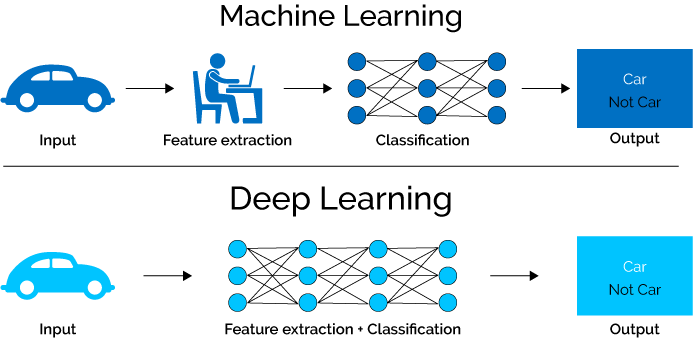
\includegraphics[width=\textwidth]{img/Caratteristiche-e-funzionamento-del-Deep-Learning-in-informatica.png}
    \captionof{figure}{Esempio comparativo tra funzionamento Machine Learning e Deep Learning}
    \url{https://goodboychan.github.io/images/copied_from_nb/image/fe.png}
    \label{fig:ml_dl_example}
\end{minipage}

Tuttavia, in molti settori, specialmente nella medicina e in altre 
discipline correlate, è difficile ottenere un insieme di dati 
sufficientemente ampio e diversificato per applicare queste tecniche. 
In questi contesti, i modelli meccanicistici rimangono la scelta 
principale. L'approccio data-driven dei modelli di machine learning, 
tuttavia, offre maggiore flessibilità e la possibilità di evitare 
ipotesi semplificative richieste dai modelli teorici.

Un'Equazione Differenziale Universale (UDE) è definita da un 
"approssimatore universale", un oggetto parametrico in grado di 
rappresentare qualsiasi funzione dati un certo numero di parametri. 
Gli approssimatori universali includono, ad esempio, le serie di Fourier 
o di Chebyshev per spazi a basse dimensioni e le reti neurali per spazi 
ad alta dimensione \cite{rackauckas2020universal}.

Un'UDE è un sistema di equazioni differenziali o algebriche non triviali 
che può approssimare qualsiasi funzione continua su un intervallo a 
qualsiasi livello di precisione desiderato. In altre parole, un'UDE è 
in grado di rappresentare qualsiasi sistema dinamico continuo con 
qualsiasi grado di dettaglio richiesto.

L'approccio delle UDE può essere accoppiato con tecniche data-driven, 
come l'algoritmo SINDy (Sparse Identification of Non-linear Dynamics), 
per l'identificazione sparsa di dinamiche non lineari in sistemi 
complessi come dinamiche dei fluidi o reti biologiche \cite{datadrivendiffeq}.

\begin{minipage}{\linewidth}
    \centering
    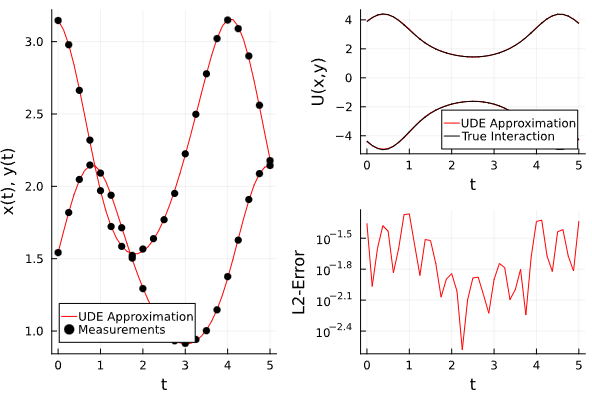
\includegraphics[width=\textwidth]{img/ude_approx.png}
    \captionof{figure}{Comportamento UDE nell'approssimazione di fenomeni non lineari \cite{rackauckas2020universal}}
    \label{fig:UDE_approx}
\end{minipage}